% !TeX root = ../thuthesis-example.tex

\chapter{引言}
\label{introduction}
对大部分的无人系统而言,为了让其能够自主完成任务,任务通常被分解为感知、决策、控制三个子任务,并要求在任务过程中有稳定的定位和通信。四旋翼飞行器是一种具有敏捷动作能力的飞行器,考虑到实际应用场景,飞行器往往需要具备自主感知和决策的能力以摆脱对外部定位、通信和操纵的依赖。在这种情况下四旋翼飞行器的自主导航是极具挑战性的系统问题。本研究借助强化学习这一交互式学习的人工智能算法,提出了一种三段式训练方法以解决复杂环境下四旋翼飞行器的自主导航问题,提升算法收敛速度,提高算法泛化性和飞行稳定性。同时本研究还针对算法训练和实机部署的需求开发了一整套仿真、部署平台。

下面将详细介绍研究背景,提出三个该领域现存的主要挑战并引出研究内容。最后介绍本研究报告各章节的构成。

\section{研究背景}
\label{background}
\subsection{四旋翼飞行器发展背景}
四旋翼飞行器(quadrotor aircraft)是用四个旋翼产生升力的多轴飞行器,是直升机的一种。随着惯性测量单元(Inertial measurement unit, IMU)、飞行控制器(Flight control unit, FCU)和电子调速器(Electronic speed control, ESC)等电子器件的出现,四旋翼飞行器开始使用电传操纵系统控制,并逐渐发展为一种结构简单使用方便的飞行平台。四旋翼飞行器是迄今为止最为灵活、敏捷的无人飞行器之一\cite{verbeke2018experimental}\cite{ackermann2020ai}。得益于其敏捷的动力学特性,它们可以穿越复杂地形到达人类和大型机械无法到达的地方。四旋翼飞行器已经在搜索救援、物流、基础设施、娱乐、农业甚至军事领域得到了了广泛的应用。例如,美国国防部高级研究计划局(DARPA)在具备自主行动的无人机(集群)方向就先后设立了面向GPS拒止环境下的快速轻量级自主无人机(FLA)、面向未来复杂城市环境作战的进攻型机器人集群战术系统(OFFSET)、人机分层协作作战体系(ACE)等项目\cite{darpa2023}。

相较于其它无人系统,四旋翼飞行器在执行自主任务时具有以下三个显著特点:
\begin{enumerate}
  \item 载荷资源受限。四旋翼飞行器作为一种空中无人平台,在任务目标和续航时间确定的情况下,其载荷资源受严格限制。飞行器所搭载的传感、计算、通信设备受载荷限制影响,其提供的感知、通信质量往往比其他无人系统更低。
  \item 计算资源受限。在载荷首先的前提下,机载计算机的规模严格受限,同时考虑到功率的限制,机载计算机的计算能力往往远低于同一时代的消费级计算机。
  \item 动力学高度复杂。相较于无人车和其它飞行器,四旋翼无人机的动力学高度复杂且非线性。同时由于其飞行特性,四旋翼无人机对决策、控制的稳定性和连续性都有较高要求。
\end{enumerate}
在上述情况下,自主导航任务对算法提出了更高要求,感知算法需要对传感器噪声、运动带来的模糊和不断变化的环境具有鲁棒性,而决策和控制算法需要在包含噪声的感知结果下利用有限的计算资源做出稳定而有效的规划。现有较成熟的方法可大致分为两类:基于优化的方法和基于学习的方法,详细的介绍将在\ref{related_works}节中展开。

\subsection{强化学习发展背景}
强化学习(Reinforcement learning, RL)是机器学习的一个分支。其工作流程是智能体(Agent)在与环境(Environment)交互的过程中不断获得奖励(Reward),通过试错的方式学习到最优策略(Policy)。其工作原理如图\ref{fig_RL}所示。深度学习(Deep learning, DL)具有学习特征表示的梯度信息,而强化学习算法可以利用环境信息产生梯度并学习最佳策略。二者结合的方法被称为深度强化学习,已在各个领域取得了很多成就。例如2016年谷歌开发的AlphaGo\cite{silver2016mastering}在围棋人机大赛中战胜世界冠军李世石,标志着人工智能又一里程碑式的胜利。而后该团队推陈出新,提出了在不使用人类棋局数据情况下战胜AlphaGo的AlphaZero\cite{silver2017mastering}、在StarCraft \uppercase\expandafter{\romannumeral2}中战胜职业玩家的AlphaStar\cite{vinyals2019grandmaster}、可以预测蛋白质结构的AlphaFold\cite{senior2020improved}、可以高效计算矩阵乘法的AlphaTensor\cite{fawzi2022discovering}等AI。同时,深度强化学习在无人驾驶、机器人控制等领域也取得了很多成果\cite{chiang2019learning}\cite{liu2022safe}。后续强化学习还产生了多个分支,例如多智能体强化学习、安全强化学习等。
\begin{figure}
  \centering
  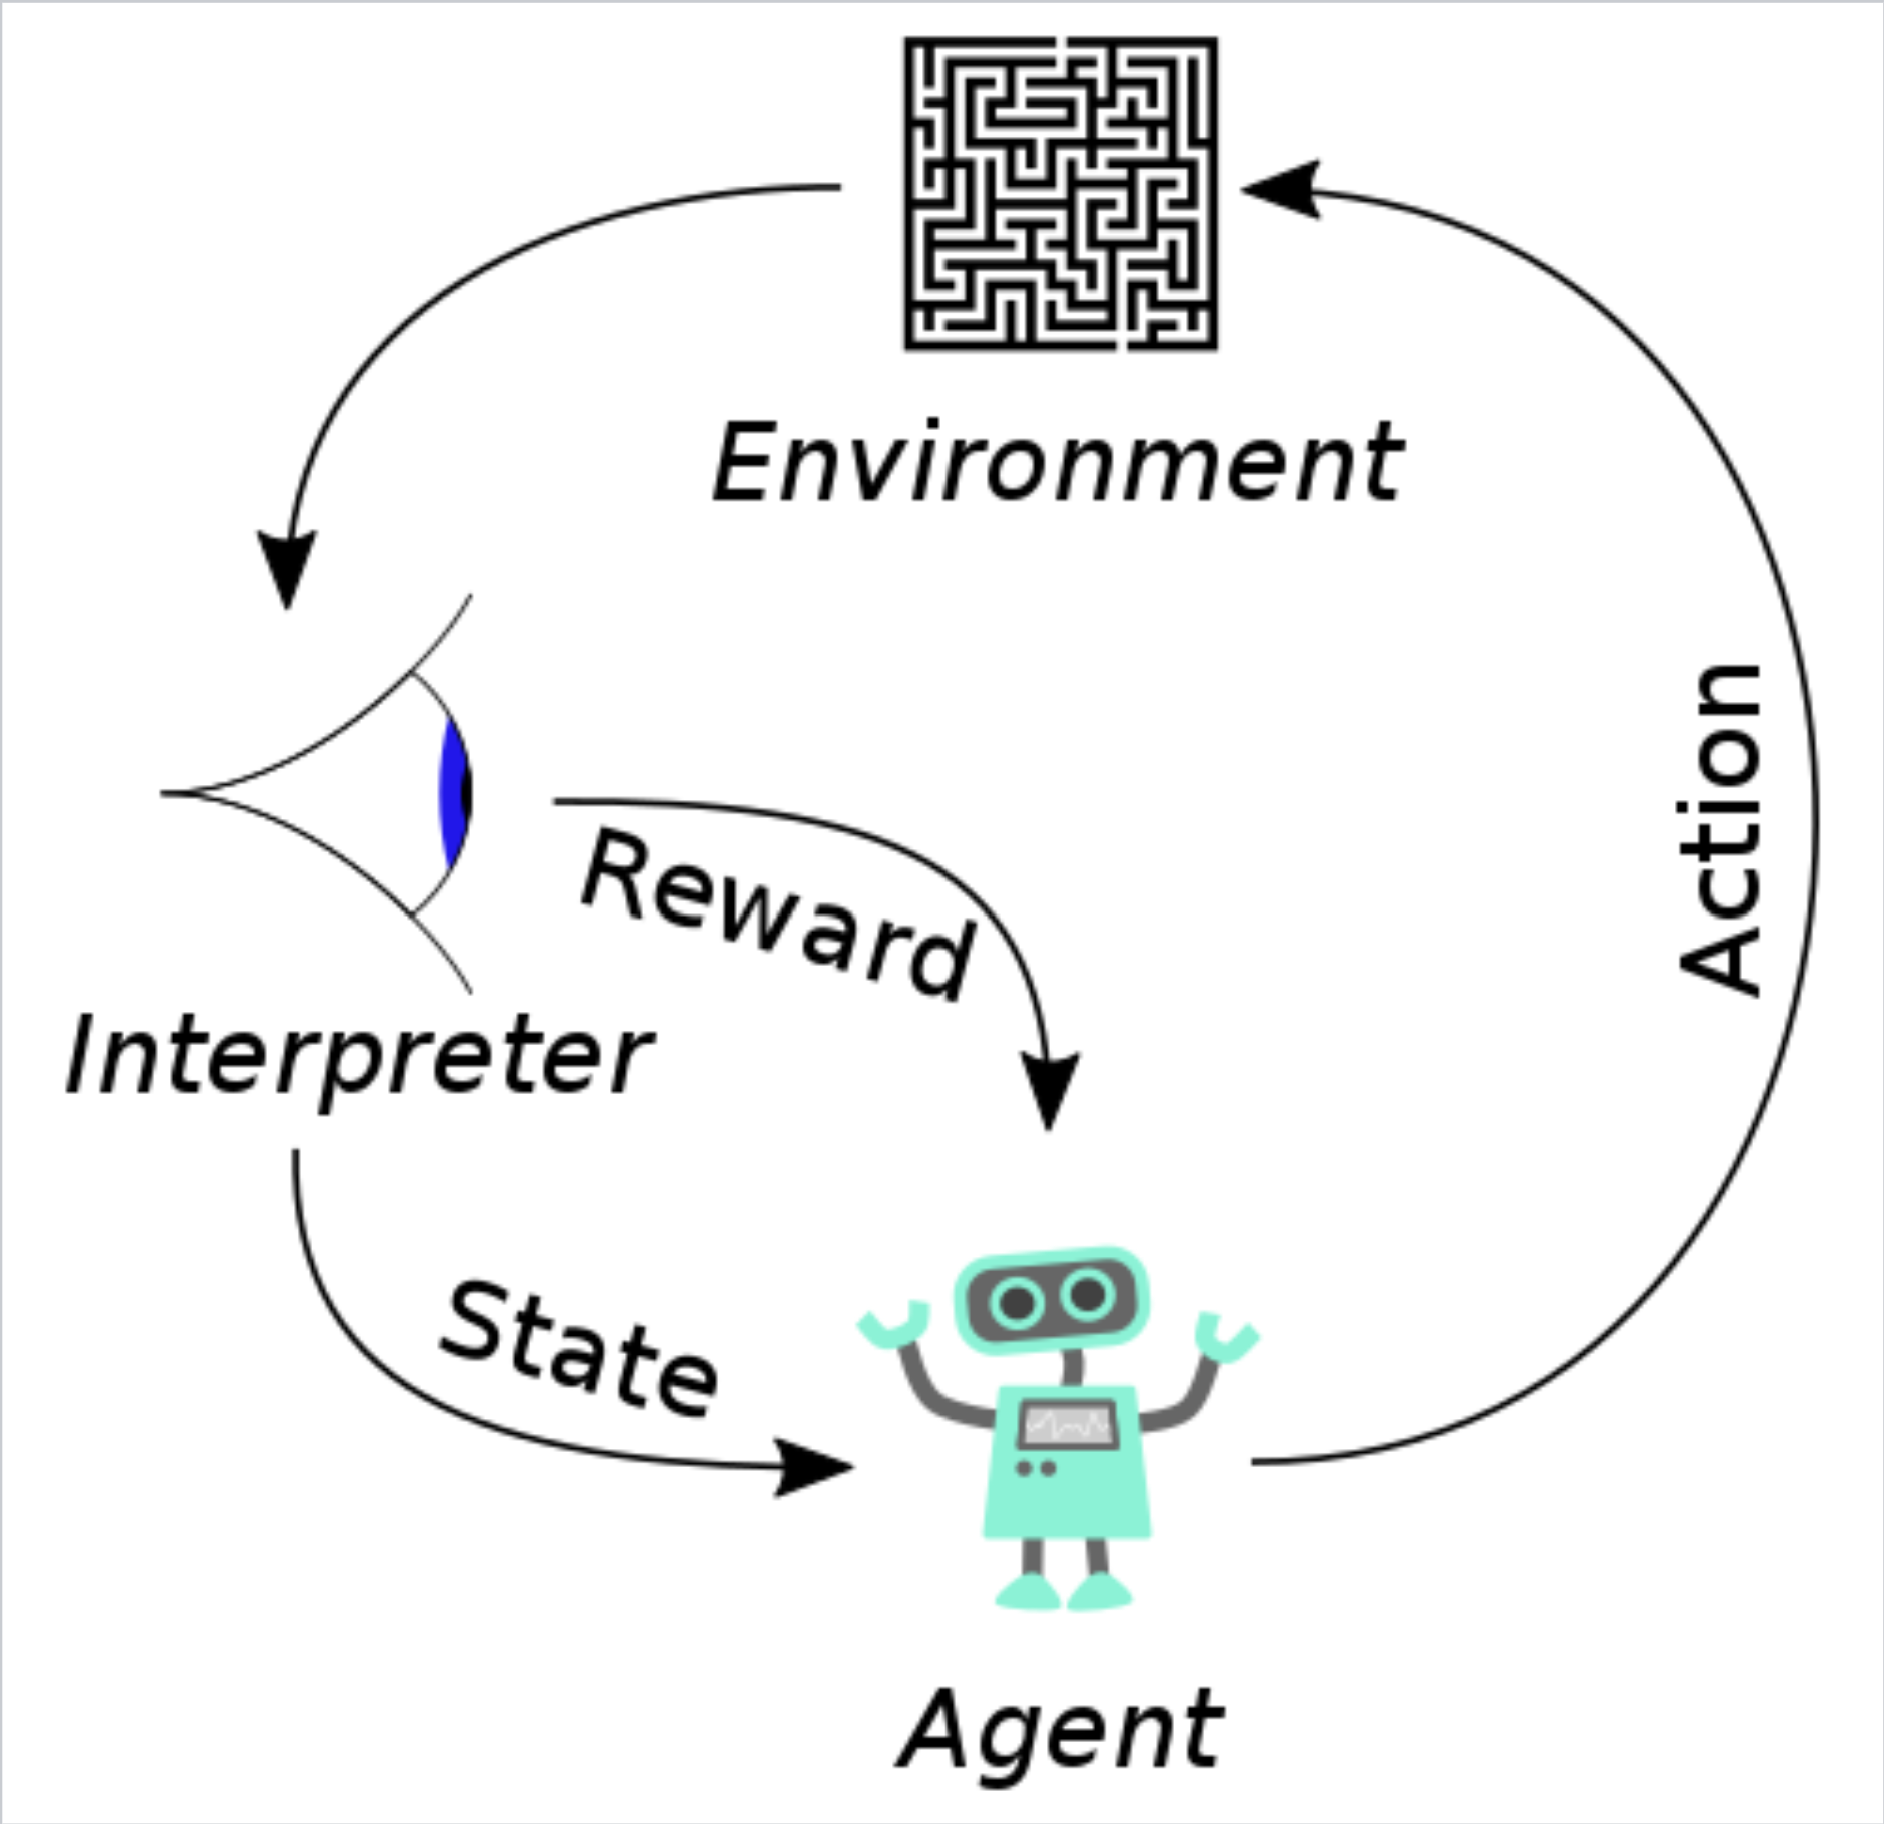
\includegraphics[width = 0.6\textwidth]{RL.png}
  \caption{强化学习工作原理}
  \label{fig_RL}
\end{figure}

\section{相关工作}
\label{related_works}
\subsection{自主导航算法}
四旋翼飞行器自主导航算法的研究已有较多成果,大体上看可以分为两类:基于优化的规划方法和基于学习的规划方法。下面将分别介绍这两类方法的研究现状。
\subsubsection{基于优化的规划方法}
同一般的无人系统一样,自主导航任务被划分为感知、规划、控制三个阶段。感知算法的任务是从传感器原始输入(如深度相机、激光雷达等)构建地图。现有的一些工作提出了从较低精度感知数据构建较高精度地图的方法\cite{heng2014autonomous}\cite{saeedi20173d}\cite{faessler2016autonomous}。而另一部分工作专注于规划无碰撞的路径而不考虑感知精度\cite{allen2016real}\cite{liu2018search}。近年来很多工作提出将这些在线建图和规划算法结合的系统,以实现在未知环境中的导航任务。例如,提出快速构建欧基里得符号距离场(Euclidean Signed Distance Fields, ESDFs)的VoxBlox\cite{oleynikova2017voxblox}、使用局部规划以提升规划效率的FASTER\cite{tordesillas2019faster}、无需构建ESDFs的规划方法EGO-Planner\cite{zhou2020ego}、考虑多无人机协同规划的EGO-swarm\cite{zhou2021ego}等。

从工程上看将导航任务分为感知、规划和控制三个子任务有不少优点:例如系统可以在不同子任务间实现并行、利用建图和规划的阶段性结果使整个系统更具可解释性等。但是三个子任务独立进行的方式忽略了不同子任务间的影响,带来了可能的累计误差,同时他们的顺序性(即下一阶段的输入为上一阶段的输出)引入了额外的延迟,为高速敏捷的飞行带来了困难\cite{falanga2019fast}。

\subsubsection{基于学习的规划方法}
总结上述工作,受限于机载计算资源和传感器精度,低延迟和高精度的感知和规划往往难以兼顾\cite{falanga2019fast}。近年来一些工作提出直接从数据中学习端到端策略而无需区分明确的感知和规划阶段。这些策略是通过模仿人类在仿真器\cite{sadeghi2016cad2rl}\cite{loquercio2021learning}或现实世界\cite{gandhi2017learning}中收集的经验训练得到的。最近的工作表明在仿真器中训练得到的敏捷的规划和控制策略可以被零成本(Zero-Shot)地迁移至部署平台\cite{kaufmann2020deep}\cite{loquercio2021learning}。但此类方法需要大量经验性的人工数据或是\cite{sadeghi2016cad2rl}或是设计复杂的专家(Expert)方法以采集足够数量的训练数据\cite{loquercio2021learning}。

\subsection{仿真器}
为加快开发速度、降低试验成本,上述两类方法均需要真实可靠的仿真器作为训练、验证的工具。尤其是随着深度强化学习技术发展,使用具有更强建模能力的基于深度学习技术的方法成为了无人系统领域的未来趋势。对于以四旋翼飞行器为代表的无人系统仿真器主要有以下三点需求:
\begin{enumerate}
  \item 仿真器能够较为真实地遵循机器人自身的物理动力学定律,并能高效地解算机器人和环境产生的交互作用。
  \item 仿真器能够集成IMU、相机、轻微系统、激光雷达等传感器。因为,这些传感器普遍应用于各项无人系统中。
  \item 仿真器能够和机器人操作系统(Robot operating system, ROS)的生态系统进行对接。ROS作为当今最完善的机器人软件系统,已经成为了标准的开发机器人应用的主流工具。
\end{enumerate}
国内外已有的针对无人机的仿真器主要有以下三个:

微软(Microsoft)公司于2017年提出了AirSim无人机驾驶自动控制仿真平台\cite{airsim2017},可实现基于虚幻引擎的无人机驾驶自动控制仿真功能。同时具备普通相机,立体相机,激光雷达,全球定位系统(GPS),IMU,磁力计等传感器。

苏黎世联邦理工学院提出了Flightmare四旋翼飞行器仿真平台\cite{flightmare},由两个主要组件组成:基于Unity的渲染引擎和可用于动力学模拟的物理引擎。且两个组件完全解耦、可以独立运行。该仿真器支持ROS环境,平台上集成了丰富的传感器,包括普通相机,立体相机,IMU等。

多伦多大学提出了Gym-pybullet-drones四旋翼飞行器仿真平台\cite{pybullet},同样集成了普通相机,立体相机,IMU等的传感器,可实现无人机集群的模拟,同时支持与ROS2系统通信。

三者采用了不同的物理引擎和和界面渲染,都支持ROS、视觉传感器模块,且考虑了空气动力学因素。但是三者的仿真运行速度较慢,仿真每秒状态数(Frame per second, FPS)$<100$。难以满足强化学习等需要大量仿真数据算法的需求。

\subsection{部署平台}
四旋翼飞行器部署平台具有结构相对简单、成本相对较低的优点。常见的科研用四旋翼无人机平台,如Crazyfile\cite{crazyfly},具有结构简单、结实耐用的优点,但并不搭载感知和计算单元,依靠上位机完成整个任务流程。此类平台常用于做科研算法快速验证而无法实际部署应用,如图\ref{fig_crazyfile}所示。最近一些无人系统工作选择将其仿真平台硬件开源\cite{zhou2020ego},但其部署平台和部署系统接口高度定制化,难以二次开发,如图\ref{fig_egofly}。一些国内外公司专门研发了科研用无人机\cite{amove},但其商品化程度高,飞行性能低,不便有效的改装和定制,如图\ref{fig_amove}。
\begin{figure}
  \centering
    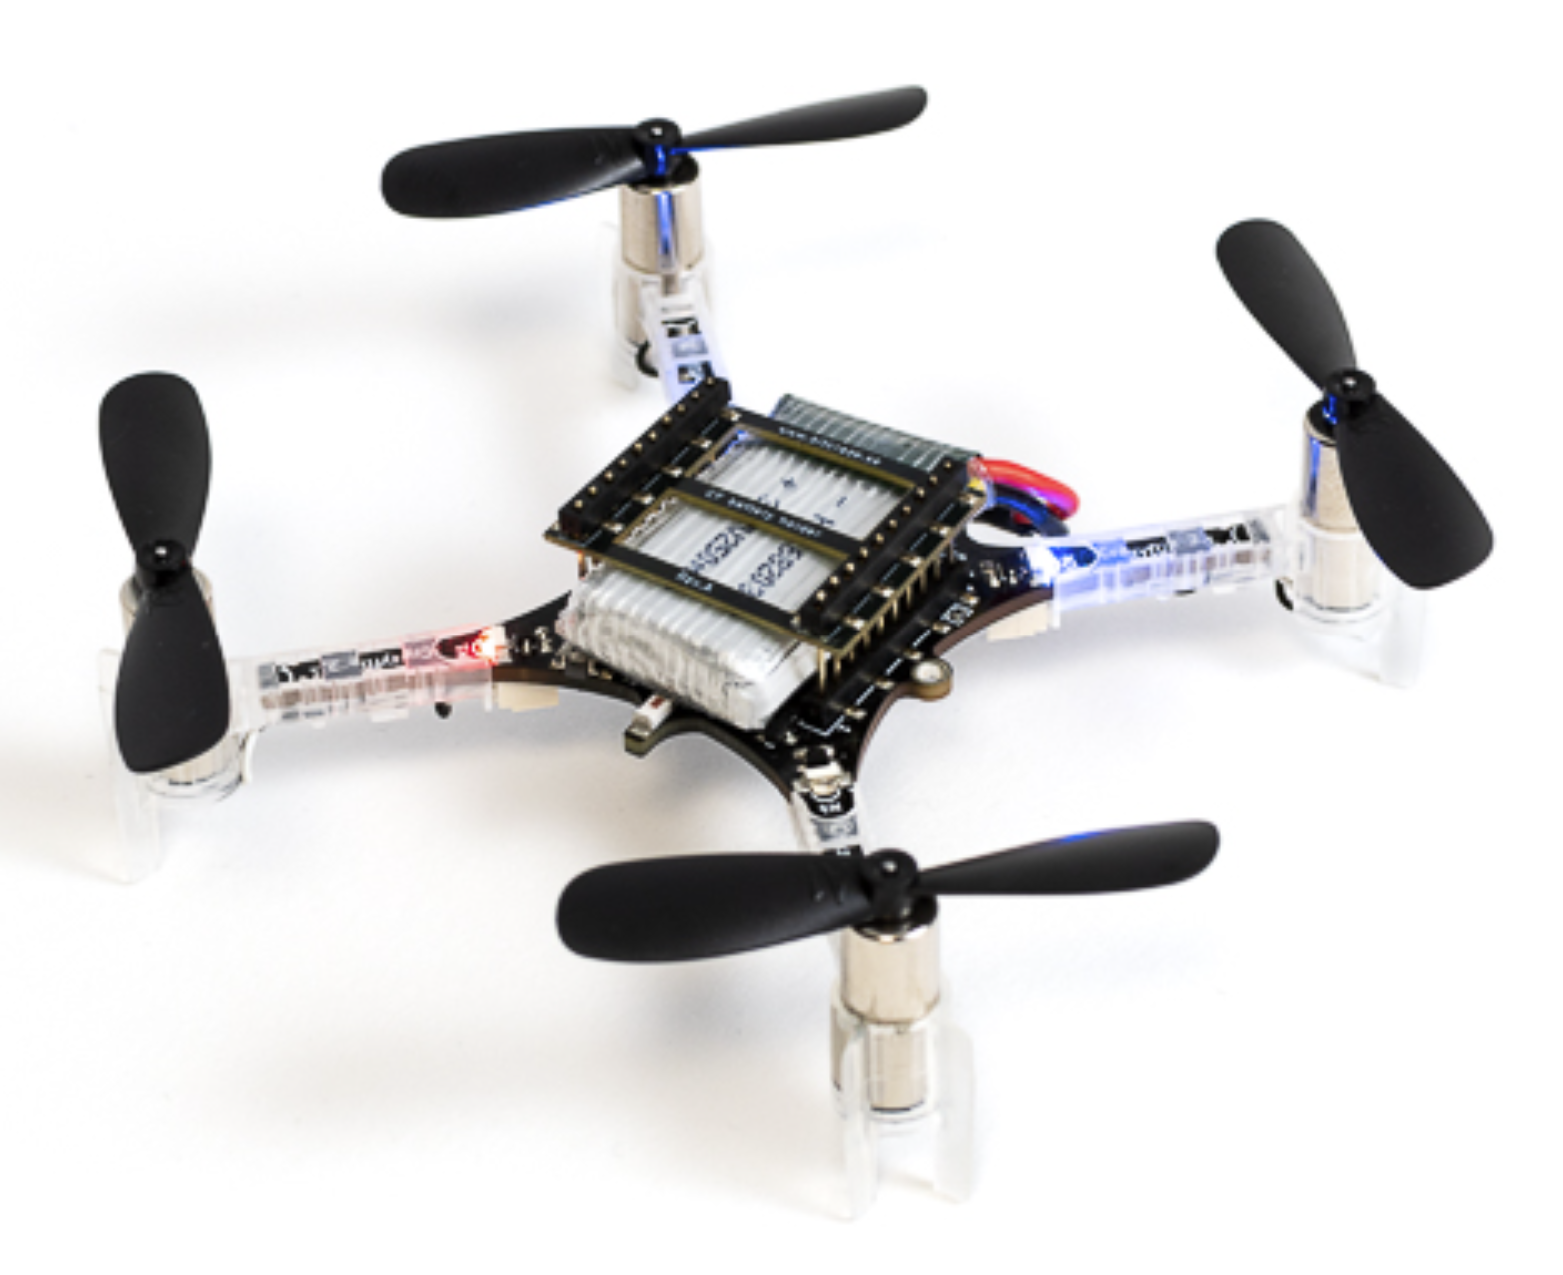
\includegraphics[width = 0.6\textwidth]{crazyfile.png}
    \caption{Crazyfile无人机}
    \label{fig_crazyfile}
\end{figure}
\begin{figure}
  \centering
    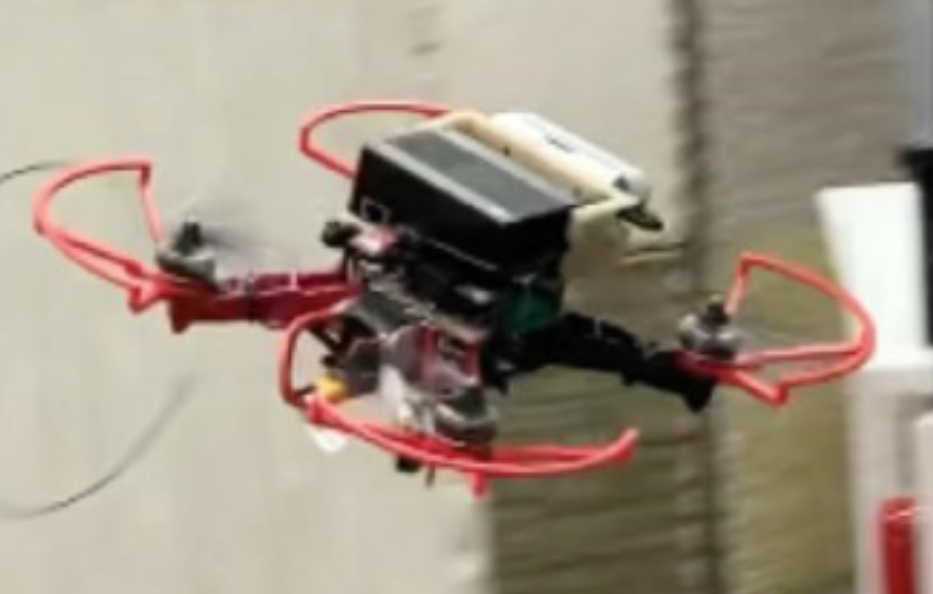
\includegraphics[width = 0.6\textwidth]{egofly.png}
    \caption{ego-planner项目硬件开源的无人机}
    \label{fig_egofly}
\end{figure}
\begin{figure}
  \centering
    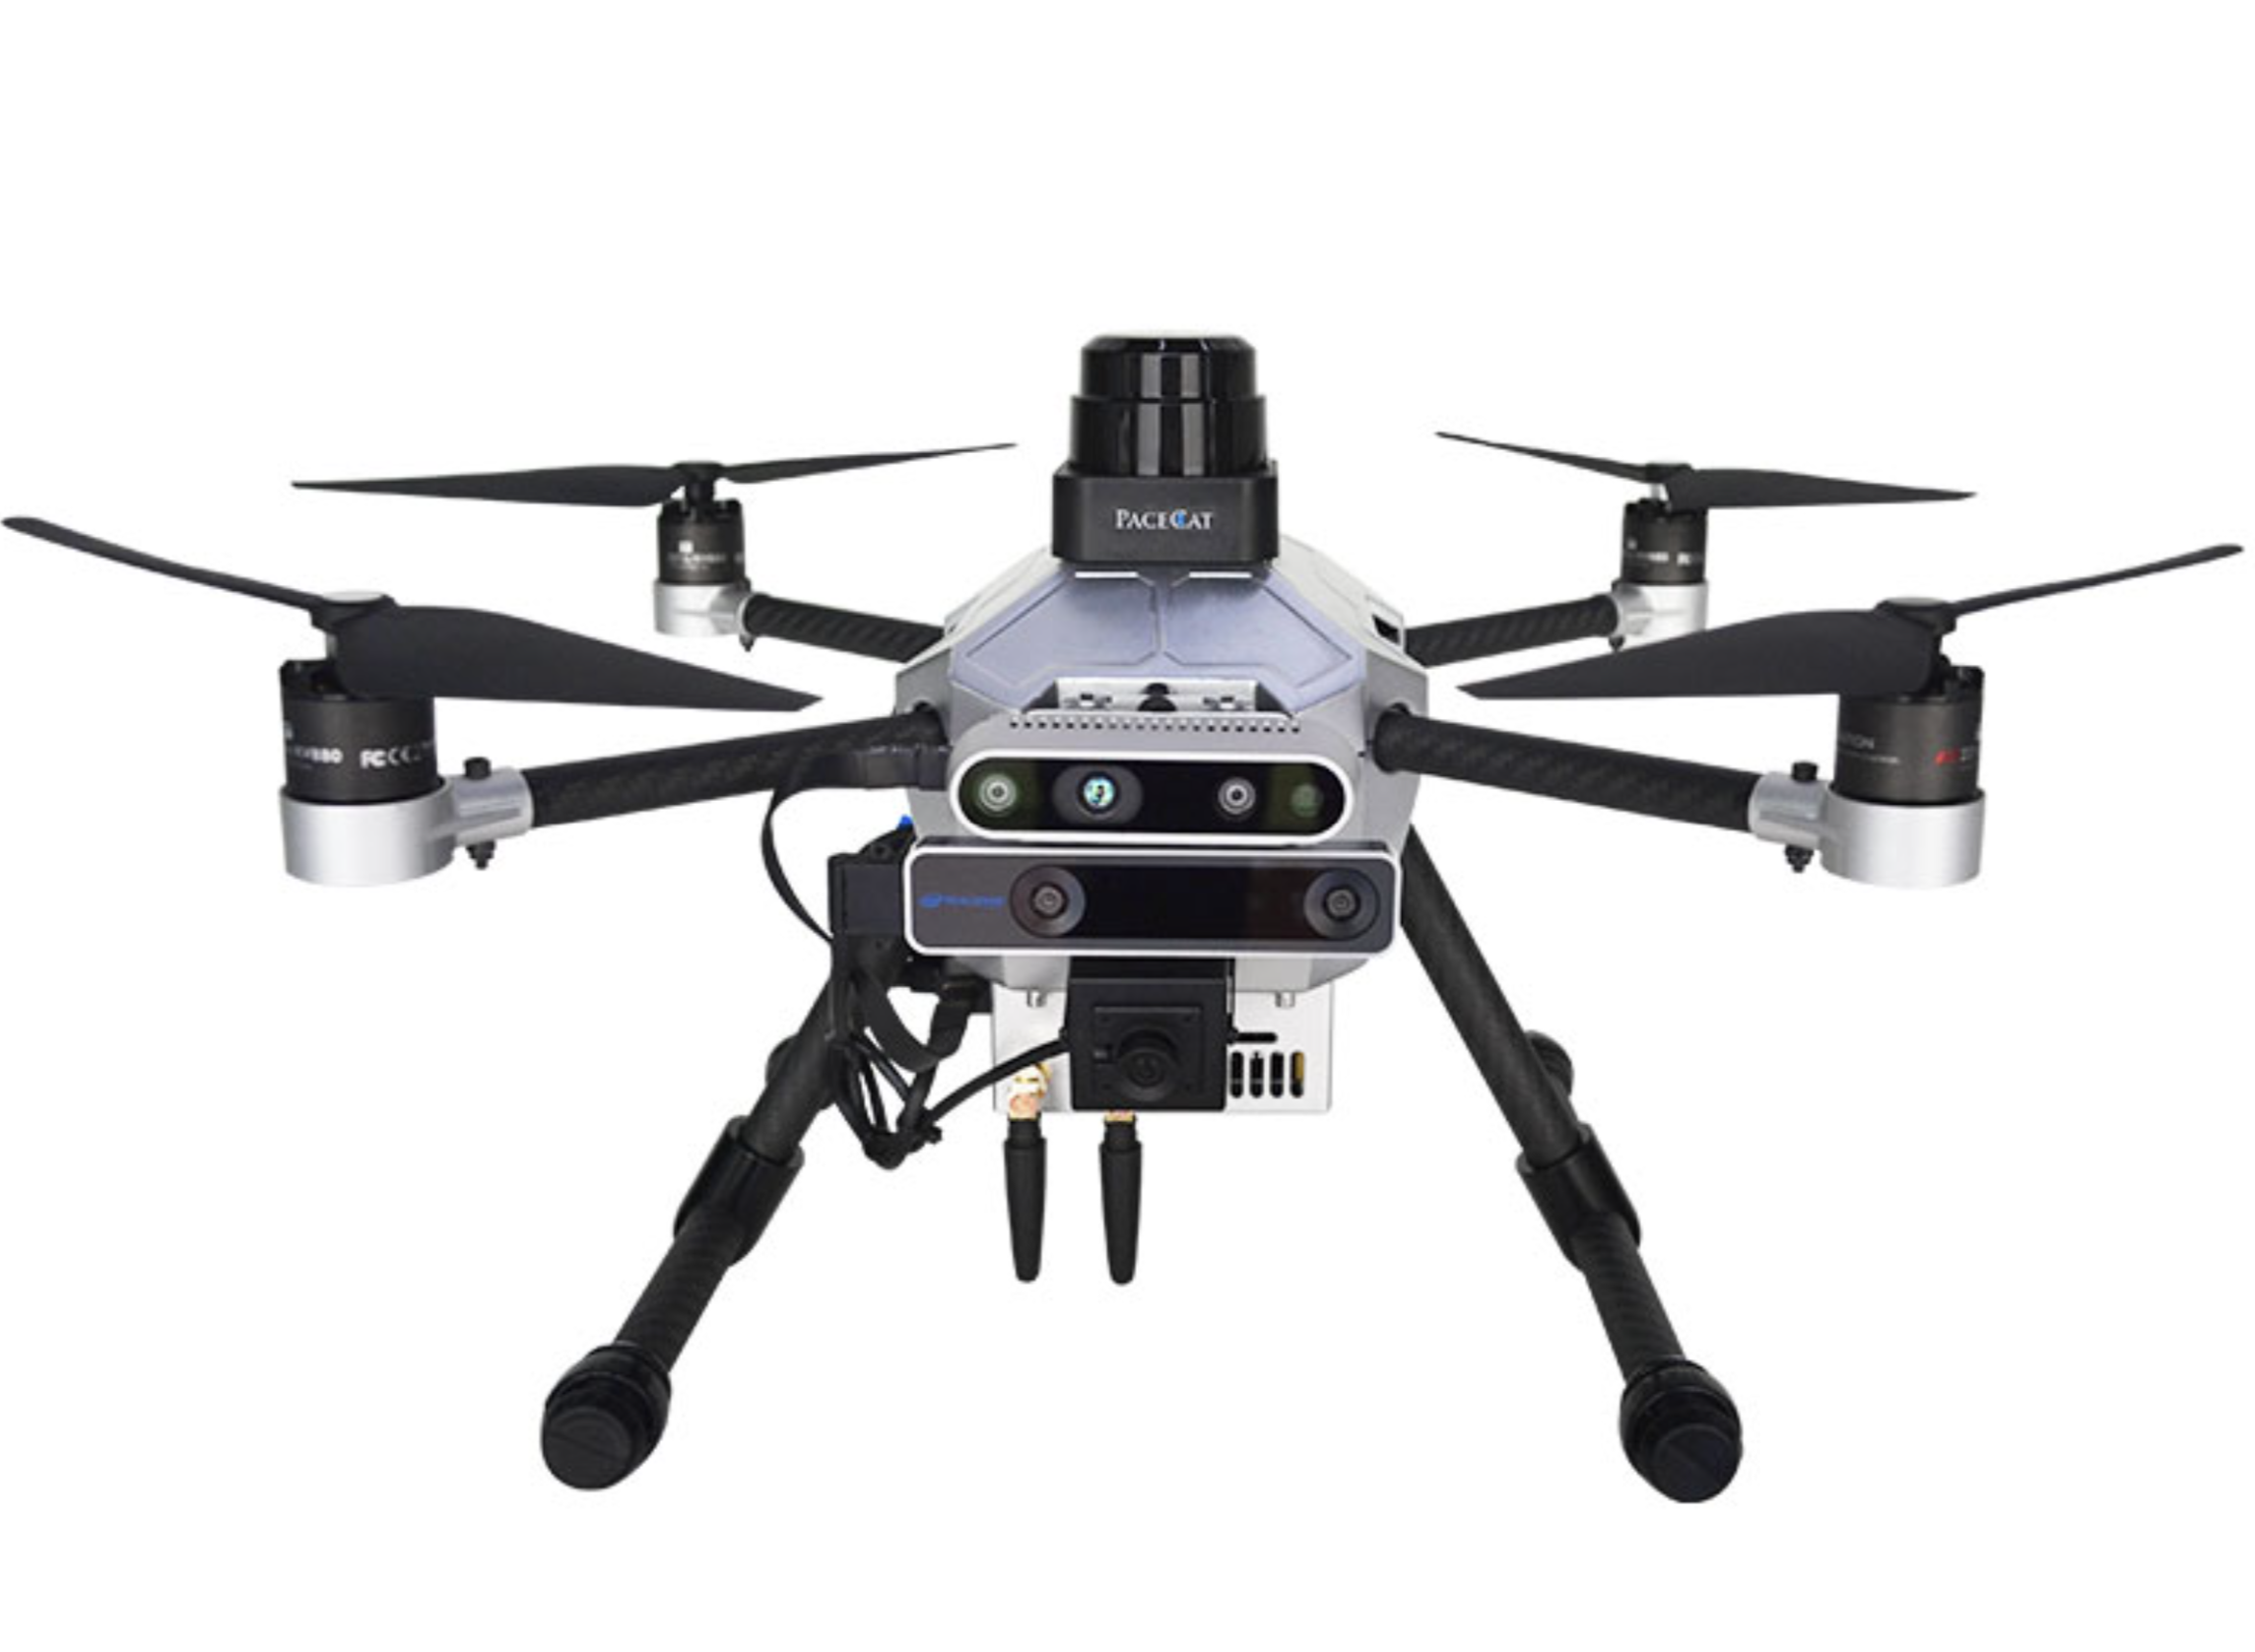
\includegraphics[width = 0.6\textwidth]{amove.png}
    \caption{市售科研用无人机}
    \label{fig_amove}
\end{figure}

\section{研究目的}
\label{target}
总结\ref{background}和\ref{related_works}节中提到的需求和研究现状,以四旋翼飞行器为代表的无人机完成自主导航任务存在以下三个挑战:
\begin{enumerate}
  \item 常用的无人机仿真器存在拟真度和仿真速度的矛盾。根据调研和实验,拟真度较高的仿真器虽然可以实现零成本部署,但采集数据速度慢,采集一条轨迹数据需要约90s时间\cite{loquercio2021learning}。而采集数据速度较快的仿真器往往难以直接部署\cite{zhu2022viola}。
  \item 现存的无人机自主导航算法难以满足需求。基于感知算法的使用优化方法的规划器规划速度慢,算力需求高\cite{ren2022bubble}。而基于人类专家数据的深度学习方法虽然很好的解决了规划速度的问题,但需要较大量的人类专家数据\cite{loquercio2021learning},需要大量经验性的设定。
  \item 目前尚没有一种功能齐全、接口丰富、运行稳定的成熟的无人机平台供自主导航任务使用。
\end{enumerate}

本研究聚焦无人机在无外部定位、通信、操纵情况下的自主导航任务。对应于上述三个挑战,主要研究内容有三:
\begin{enumerate}
  \item 基于现有仿真器,通过增加并行度等方法提高仿真器采集数据的速度以满足强化学习算法对大量数据的需求。
  \item 设计一种基于强化学习的无人机自主导航算法,并设计配套的训练方法。在利用强化学习算法解决算法运行速度慢、需要大量专家数据这两个问题的同时也尽可能规避其自身存在的数据效率低、收敛慢等问题。
  \item 设计并搭建具有自主定位、自主计算的四旋翼无人机并设计一套部署系统。该部署系统应集成多种传感器和多种控制器供选择,并预留完善的算法接口。最后在该算法平台上验证自主导航算法的实际飞行效果。
\end{enumerate}
本研究的研究框架如图\ref{fig_outline}所示。
\begin{figure}
  \centering
  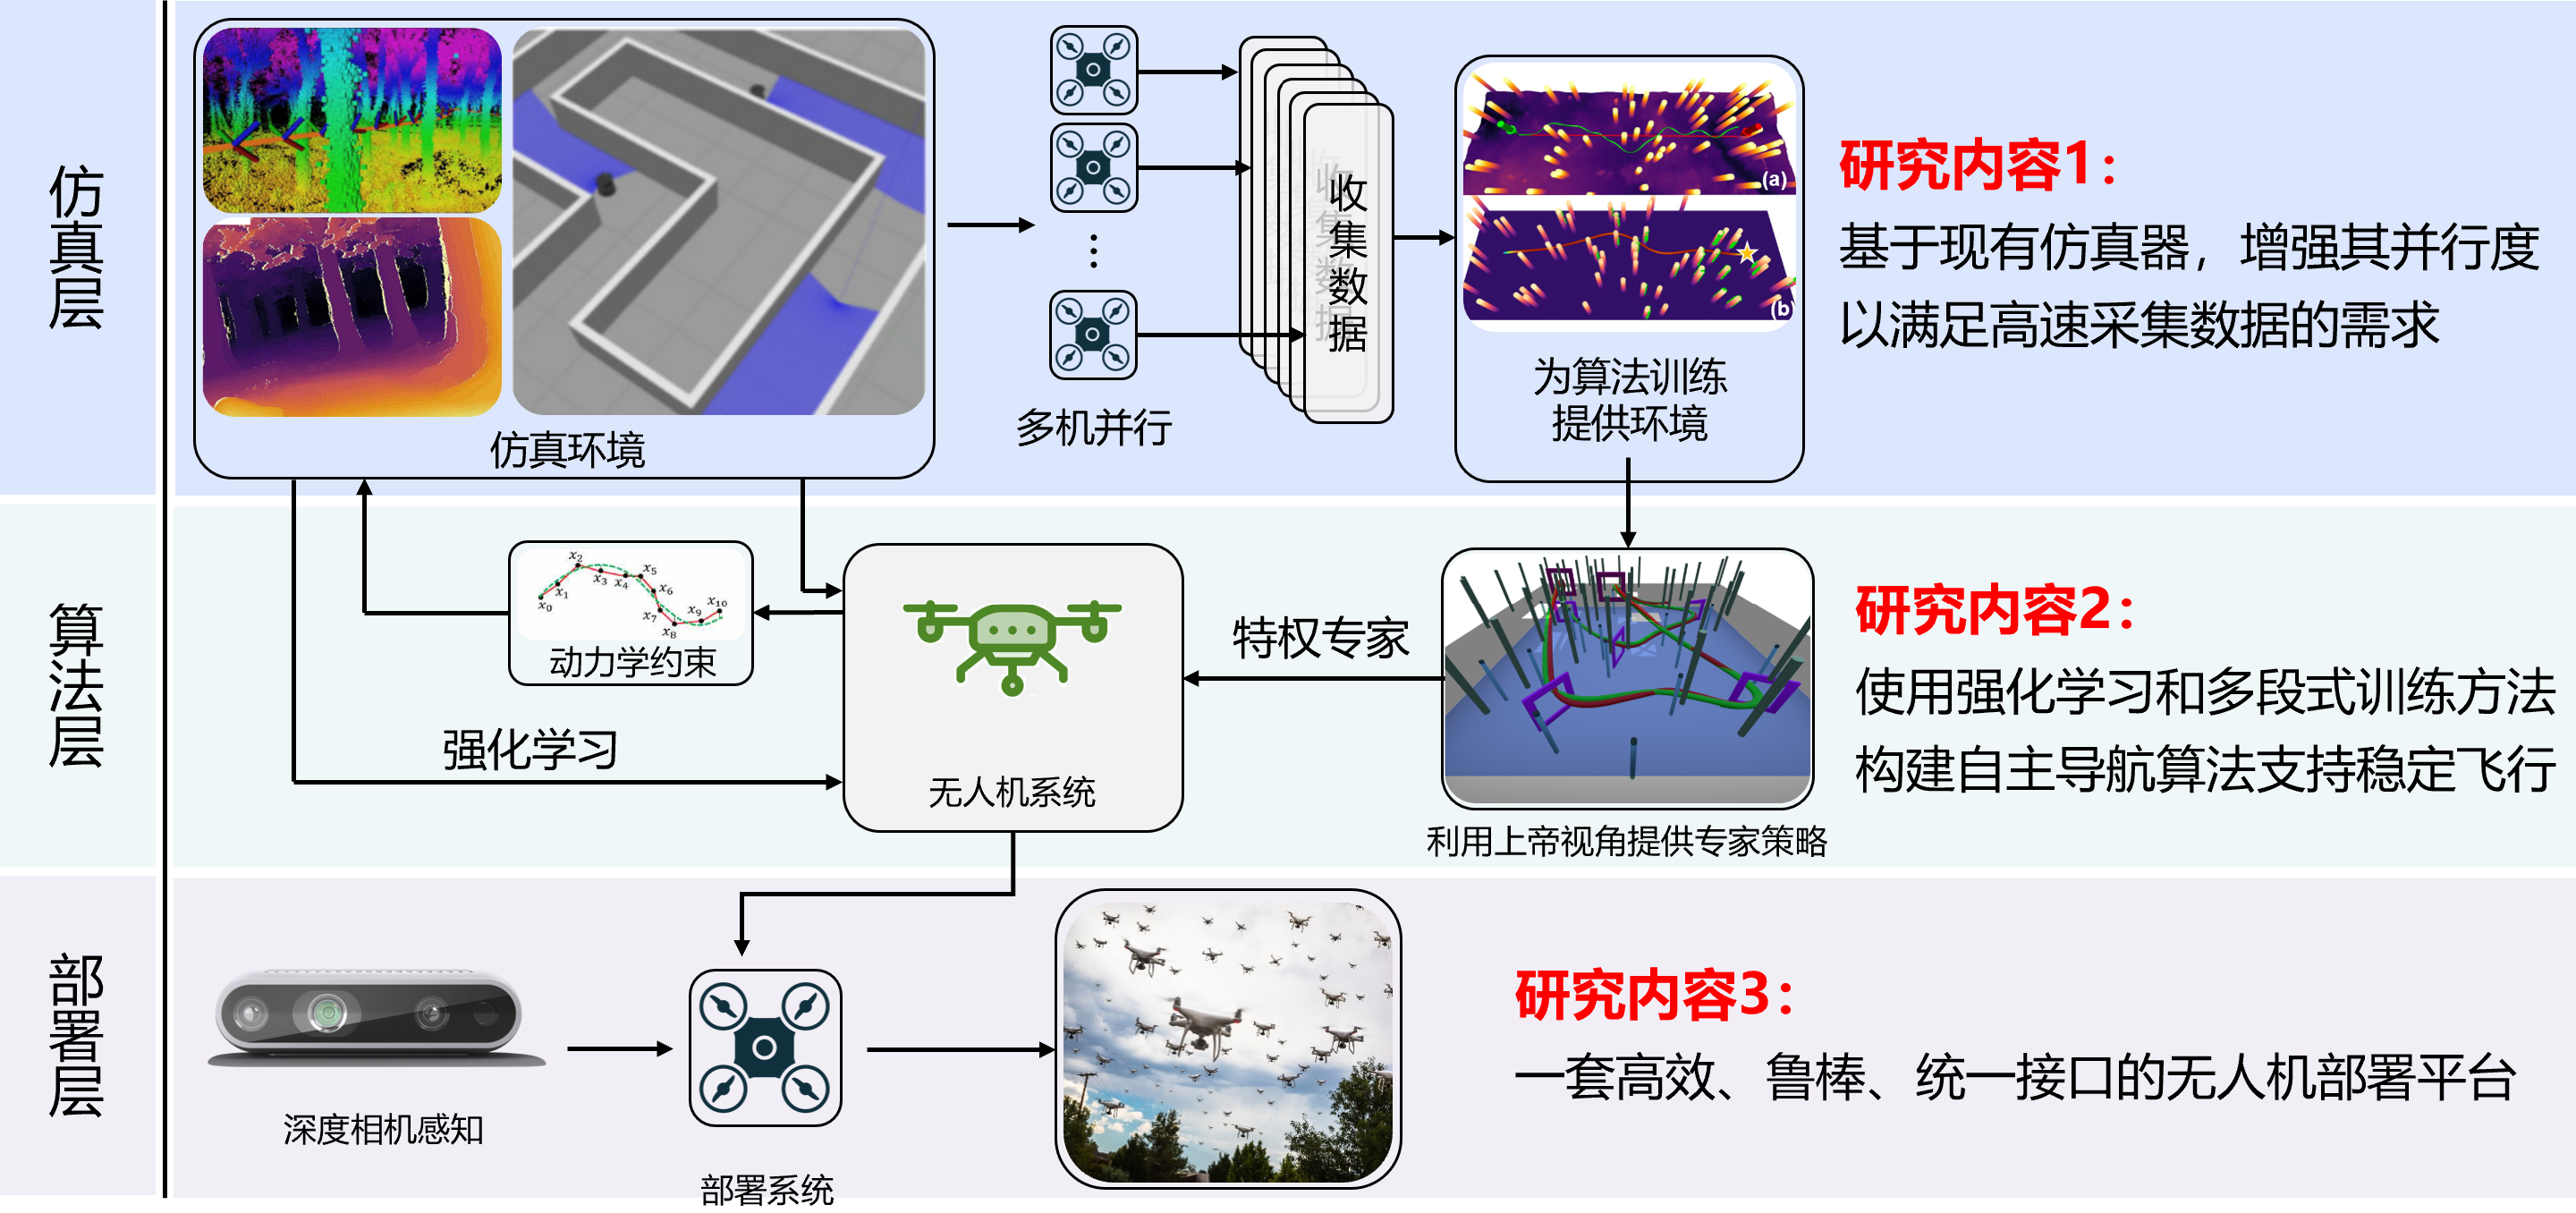
\includegraphics[width = 1\textwidth]{outline.png}
  \caption{研究框架示意图}
  \label{fig_outline}
\end{figure}

本研究是一个系统性研究,其中强化学习算法设计部分为主要的创新点。仿真器和部署平台包含则较多工程技巧,工作量较大,但这是完成算法训练和算法验证必不可少的环节。同时本项目所设计的仿真器和部署平台将作为课题组后续相关研究重要的基础设施。

\section{各章节概述}
\label{outline}
本研究报告共分为六章,本章主要介绍了本研究的背景、现存挑战,从应用和学术研究的角度阐述了本研究的必要性和挑战性。第二章至第四章分别介绍了仿真器的改进工作、强化学习算法和部署平台的结构设计,并简要介绍这些设计对总体飞行性能的影响。第五章介绍了本研究的实验结果,包括仿真平台参数的设置,算法调试的结果和实机部署的结果。第六章对本研究做一个整体总结并提出该项目未来可继续改进的方向。


% \section{引言的写法}

% 一篇学位论文的引言大致包含如下几个部分:
% 1、问题的提出;
% 2、选题背 景及意义;
% 3、文献综述;
% 4、研究方法;
% 5、论文结构安排。
% \begin{itemize}
%   \item 问题的提出:要清晰地阐述所要研究的问题“是什么”。
%     \footnote{选题时切记要有“问题意识”,不要选不是问题的问题来研究。}
%   \item 选题背景及意义:论述清楚为什么选择这个题目来研究,即阐述该研究对学科发展的贡献、对国计民生的理论与现实意义等。
%   \item 文献综述:对本研究主题范围内的文献进行详尽的综合述评,“述”的同时一定要有“评”,指出现有研究状态,仍存在哪些尚待解决的问题,讲出自己的研究有哪些探索性内容。
%   \item 研究方法:讲清论文所使用的学术研究方法。
%   \item 论文结构安排:介绍本论文的写作结构安排。
% \end{itemize}



% \section{正文的写法}

% 本部分是论文作者的研究内容,不能将他人研究成果不加区分地掺和进来。
% 已经在引言的文献综述部分讲过的内容,这里不需要再重复。
% 各章之间要存在有机联系,符合逻辑顺序。



% \section{结论的写法}

% 结论是对论文主要研究结果、论点的提炼与概括,应精炼、准确、完整,使读者看后能全面了解论文的意义、目的和工作内容。
% 结论是最终的、总体的结论,不是正文各章小结的简单重复。
% 结论应包括论文的核心观点,主要阐述作者的创造性工作及所取得的研究成果在本领域中的地位、作用和意义,交代研究工作的局限,提出未来工作的意见或建议。
% 同时,要严格区分自己取得的成果与指导教师及他人的学术成果。

% 在评价自己的研究工作成果时,要实事求是,除非有足够的证据表明自己的研究是“首次”、“领先”、“填补空白”的,否则应避免使用这些或类似词语。
